\documentclass[12pt]{article}
\usepackage[utf8]{inputenc}
\usepackage[margin=1in]{geometry}
\usepackage{booktabs}
\usepackage{graphicx}
\usepackage{hyperref}
\hypersetup{hypertexnames=false}
\usepackage{enumitem}
\usepackage{amsmath}
\usepackage{float}

\title{\textbf{Determinants of Household Stock Market Participation in Italy}\\
\large Evidence from the 2022 Survey on Household Income and Wealth}
\author{Murtaza}
\date{\today}

\begin{document}

\maketitle

\tableofcontents
\newpage

\begin{abstract}
This report studies why some Italian households participate in the stock market while others do not. Using the 2022 Survey on Household Income and Wealth (SHIW) from the Bank of Italy, the project examines whether household income and education predict ownership of risky financial assets such as mutual funds, ETFs, listed shares, unlisted shares, and foreign securities. The empirical strategy uses a binary dependent variable for stock market participation and estimates weighted probit models. The results show that both income and education are strong positive predictors of participation. The weighted participation rate in the final sample is 11.97 percent. University education is associated with a 13.61 percentage point higher probability of participation compared with primary education or less, after controlling for income, age, region, household size, and gender of the household head.
\end{abstract}

\section{Introduction}

Household financial decisions are important because they affect saving, wealth accumulation, retirement security, and exposure to financial risk. In theory, households with enough savings should hold diversified portfolios that include some risky financial assets, such as stocks or equity mutual funds. In practice, many households hold most of their financial wealth in safe and liquid instruments, especially bank deposits. This pattern is visible in many countries, including Italy.

The main objective of this project is to understand which household characteristics predict participation in financial markets. The central research question is:

\begin{quote}
\textbf{To what extent do household income and education predict the probability that an Italian household owns stocks, mutual funds, ETFs, or similar risky financial assets?}
\end{quote}

The project focuses on income and education for two reasons. First, income affects the ability to invest. Households with higher income are more likely to have savings left after consumption and may be more able to accept financial risk. Second, education is often related to financial literacy, access to information, and confidence in dealing with financial products.

This question is relevant for financial economics because it helps explain the stock market participation puzzle: why many households do not invest in risky assets even when long-run diversification may be beneficial. It is also relevant for banks, investment firms, and financial advisors because it helps identify groups that may be underserved by current financial products.

\subsection{Contribution of the Project}

The contribution of this project is practical and empirical. First, it translates a broad question in household finance into a concrete empirical design using real household survey data. Second, it shows how to construct a clean household-level dataset from several SHIW files. Third, it estimates and interprets a binary choice model in a way that is useful for both academic and business audiences.

The project does not claim to identify a causal effect of education or income. Instead, it provides evidence about strong predictors of participation. This distinction is important. A causal study would require an identification strategy such as a natural experiment, instrumental variable, or panel design. The present report is more modest: it asks whether income and education are systematically associated with participation after controlling for other observable household characteristics.

\section{Literature Review}

\subsection{The Stock Market Participation Puzzle}

Standard portfolio theory suggests that households should hold diversified portfolios that include some risky assets, especially when they have a long investment horizon. However, empirical studies show that many households do not own stocks directly or indirectly. This is known as the stock market participation puzzle.

Haliassos and Bertaut (1995) were among the early authors to ask why so few households hold stocks. They argued that fixed participation costs, lack of information, and background risk can help explain limited participation. If households face costs of learning about stocks, opening brokerage accounts, or choosing financial products, then low participation can be rational even when expected returns are high.

Campbell (2006) developed the broader field of household finance by emphasizing that households often make financial mistakes or avoid complex financial decisions. Stock market non-participation is one of the central examples. Households may fail to diversify, hold inefficient portfolios, borrow at high interest rates, or avoid financial markets altogether.

\subsection{Income, Wealth, and Participation}

Income and wealth are usually among the strongest predictors of financial market participation. Richer households can more easily pay fixed entry costs and are more likely to have savings beyond precautionary balances. A low-income household may rationally prefer deposits because liquidity is more important than long-run returns.

Income can also proxy for access to financial institutions. Higher-income households may have more contact with banks, investment advisors, and digital platforms. They may also receive more financial information through their work or social networks.

In this project, income is measured as household income and transformed using the natural logarithm. This is consistent with the idea that proportional changes in income are more meaningful than equal euro changes across the whole distribution. For example, an increase from EUR 20,000 to EUR 30,000 is more important for household behavior than an increase from EUR 200,000 to EUR 210,000.

\subsection{Education and Financial Literacy}

Education is another key predictor of financial market participation. More educated households may better understand compound returns, inflation, diversification, and risk. They may also be more comfortable comparing investment products and reading financial documents.

Van Rooij, Lusardi, and Alessie (2011) show that financial literacy is strongly related to stock market participation. Although this project uses formal education rather than direct financial literacy questions, education can act as a proxy for some of the cognitive and informational skills needed to participate in financial markets.

Guiso, Sapienza, and Zingales (2008) emphasize the role of trust. Even households with sufficient resources may avoid stocks if they do not trust financial institutions or the stock market. Education may matter partly because more educated households feel more able to evaluate financial information and avoid fraud or unsuitable products.

\subsection{Italian Context}

Italy is an especially interesting country for this question because household saving has traditionally been high, while direct participation in risky financial assets is limited. Italian households often hold a large share of wealth in housing and bank deposits. This makes it important to understand why only a minority of households participate in stock markets.

Regional differences are also important in Italy. The North, Centre, and South differ in income levels, employment opportunities, financial development, and household wealth. For this reason, the empirical model controls for geographic region.

\section{Conceptual Framework and Hypotheses}

\subsection{Conceptual Framework}

The decision to participate in the stock market can be understood as a comparison between expected benefits and expected costs.

The benefits include potential long-run returns, diversification, and wealth accumulation. The costs include information costs, transaction costs, risk exposure, distrust, and the psychological cost of dealing with uncertainty.

Income affects both sides of this comparison. Higher-income households are more likely to have investable savings and can absorb losses more easily. Education affects the information side. More educated households may face lower learning costs and may better understand the benefits of diversification.

The relationship can be summarized as follows:

\[
\text{Participation} =
f(\text{Income}, \text{Education}, \text{Risk Capacity}, \text{Information}, \text{Demographics}).
\]

\subsection{Hypotheses}

The project tests two main hypotheses:

\begin{itemize}[leftmargin=*]
    \item \textbf{Hypothesis 1:} Higher household income is associated with a higher probability of stock market participation.
    \item \textbf{Hypothesis 2:} Higher education of the household head is associated with a higher probability of stock market participation.
\end{itemize}

The expected signs are positive for both income and education. The model also controls for age, region, household size, and gender of the household head to reduce omitted-variable bias from observable demographic differences.

\section{Data Source}

\subsection{Survey on Household Income and Wealth}

The data come from the \textbf{Survey on Household Income and Wealth (SHIW)}, conducted by the \textbf{Bank of Italy}. The SHIW is a household-level survey containing information on income, wealth, financial assets, demographic characteristics, education, and household composition.

The files used in this project are from the 2022 SHIW Stata folder:

\begin{itemize}[leftmargin=*]
    \item \texttt{q22a.dta}: household-level information, including household size and sampling weights;
    \item \texttt{rfam22.dta}: household income variables;
    \item \texttt{q22c2.dta}: ownership of financial assets;
    \item \texttt{carcom22.dta}: individual-level demographic information, used to identify characteristics of the household head.
\end{itemize}

The household identifier used to merge the files is \texttt{nquest}. This variable uniquely identifies each household in the household-level files.

\subsection{Why These Files Were Used}

The project needs three types of information:

\begin{enumerate}[leftmargin=*]
    \item whether the household owns risky financial assets;
    \item household economic resources, especially income;
    \item demographic characteristics such as education, age, region, and household size.
\end{enumerate}

No single SHIW file contains all these variables together. Therefore, the analysis merges multiple files. The asset variables are in \texttt{q22c2.dta}, income is in \texttt{rfam22.dta}, household size and survey weight are in \texttt{q22a.dta}, and household-head education and age are in \texttt{carcom22.dta}.

\subsection{Unit of Analysis}

The unit of analysis is the household. This choice is appropriate because the SHIW measures financial assets and income at the household level. In many households, financial decisions are made jointly or are at least influenced by shared household resources. Therefore, the dependent variable measures whether the household participates, not whether a specific individual participates.

For demographic characteristics, the project uses the household head. This is a common approach in household-level empirical work. The household head's age and education summarize important socioeconomic characteristics of the household. This approach is not perfect because other household members may influence financial decisions, but it provides a consistent and interpretable measure.

\subsection{Data Dictionary}

\begin{table}[H]
\centering
\caption{Main Variables Used in the Analysis}
\begin{tabular}{lll}
\toprule
\textbf{Concept} & \textbf{Variable / Source} & \textbf{Role in Analysis} \\
\midrule
Household ID & \texttt{nquest} & Merge key \\
Income & \texttt{Y} in \texttt{rfam22.dta} & Main explanatory variable \\
Household size & \texttt{NCOMP} in \texttt{q22a.dta} & Control variable \\
Survey weight & \texttt{PESOFIT} in \texttt{q22a.dta} & Population weighting \\
Education & \texttt{STUDIO} in \texttt{carcom22.dta} & Main explanatory variable \\
Age & \texttt{ETA} in \texttt{carcom22.dta} & Control variable \\
Region & \texttt{AREA3} in \texttt{carcom22.dta} & Control variable \\
Gender & \texttt{SEX} in \texttt{carcom22.dta} & Control variable \\
Funds & \texttt{POS\_D3} in \texttt{q22c2.dta} & Dependent-variable input \\
ETFs & \texttt{POS\_D4} in \texttt{q22c2.dta} & Dependent-variable input \\
Listed shares & \texttt{POS\_E1} in \texttt{q22c2.dta} & Dependent-variable input \\
Unlisted shares & \texttt{POS\_E2} in \texttt{q22c2.dta} & Dependent-variable input \\
Foreign securities & \texttt{POS\_F2} in \texttt{q22c2.dta} & Dependent-variable input \\
\bottomrule
\end{tabular}
\end{table}

\section{Data Validation}

Before estimating the model, the data were validated to make sure the merge and variable construction were correct. This is important because empirical results are only credible if the dataset is correctly built.

\subsection{Validation Checks Performed}

The validation script checked the following:

\begin{itemize}[leftmargin=*]
    \item number of rows in each raw file;
    \item number of unique household identifiers;
    \item whether all household IDs in \texttt{q22a.dta} also appear in \texttt{rfam22.dta} and \texttt{q22c2.dta};
    \item whether every household has one household head in \texttt{carcom22.dta};
    \item whether there are duplicate household heads;
    \item whether the final analysis dataset contains missing values in required variables;
    \item whether income, age, and weights contain impossible values;
    \item whether the constructed stock participation variable exactly matches the raw asset columns.
\end{itemize}

\subsection{Validation Results}

The validation results were satisfactory. The household-level files \texttt{q22a.dta}, \texttt{rfam22.dta}, and \texttt{q22c2.dta} each contain 9,641 households. The person-level file \texttt{carcom22.dta} contains 23,057 people and 9,641 unique households, which is expected because households can have multiple members.

The final analysis dataset contains 9,617 households. The difference between 9,641 and 9,617 is due to dropping observations with invalid or missing values required for the model, especially non-positive income or missing model variables.

\begin{table}[H]
\centering
\caption{Main Data Validation Results}
\begin{tabular}{lrr}
\toprule
\textbf{Check} & \textbf{Value} & \textbf{Status} \\
\midrule
Households in \texttt{q22a.dta} & 9,641 & Pass \\
Households in \texttt{rfam22.dta} & 9,641 & Pass \\
Households in \texttt{q22c2.dta} & 9,641 & Pass \\
Unique households in \texttt{carcom22.dta} & 9,641 & Pass \\
Duplicate household heads & 0 & Pass \\
Households missing a household head & 0 & Pass \\
Final analysis sample & 9,617 & Pass \\
Missing model variables & 0 & Pass \\
Invalid income or weight & 0 & Pass \\
Participation-variable mismatches & 0 & Pass \\
\bottomrule
\end{tabular}
\end{table}

The most important validation result is that there were zero mismatches between the constructed dependent variable and the raw financial asset variables. This confirms that the main dependent variable was coded correctly.

\subsection{Why Validation Matters}

Data validation is not just a technical step. It is part of the credibility of the empirical analysis. If the merge were incorrect, the model could accidentally connect one household's income with another household's financial assets. If the household-head file contained duplicate heads, education and age could be incorrectly assigned. If the participation variable did not match the raw asset variables, the dependent variable would not answer the research question.

For this reason, the validation script is included as a separate project file. It makes the data preparation reproducible and auditable. A reader can run the script and verify that the analysis dataset is consistent with the raw SHIW files.

\section{Variable Construction}

\subsection{Dependent Variable}

The dependent variable is \texttt{stock\_participation}. It equals 1 if the household owns at least one risky financial asset and 0 otherwise. The variable is constructed from the SHIW asset ownership variables in \texttt{q22c2.dta}.

The risky financial assets used are:

\begin{itemize}[leftmargin=*]
    \item \texttt{POS\_D3}: common funds;
    \item \texttt{POS\_D4}: exchange-traded funds (ETFs);
    \item \texttt{POS\_E1}: listed company shares;
    \item \texttt{POS\_E2}: unlisted company shares;
    \item \texttt{POS\_F2}: foreign financial securities, including foreign shares and bonds.
\end{itemize}

The dependent variable is therefore:

\[
\text{stock\_participation}_i =
\begin{cases}
1 & \text{if household } i \text{ owns at least one selected risky asset,}\\
0 & \text{otherwise.}
\end{cases}
\]

This definition includes both direct stockholding and indirect stock market exposure through funds and ETFs. This is appropriate because many households participate in equity markets through investment funds instead of buying individual shares directly.

This definition is intentionally broader than direct ownership of listed stocks. If the dependent variable used only listed shares, it would miss households that participate through professionally managed products. For a household finance project, this broader definition better captures whether the household has exposure to risky financial markets.

\subsection{Main Explanatory Variables}

The two main explanatory variables are income and education.

\subsubsection{Income}

Household income comes from \texttt{rfam22.dta}, using the variable \texttt{Y}. The model uses the natural logarithm of income:

\[
\log(\text{Income}_i).
\]

The log transformation is used because income is highly skewed. A small number of households have very high income, and using log income reduces the influence of extreme values. It also allows the model to interpret income changes in proportional terms rather than in absolute euros.

\subsubsection{Education}

Education is taken from the household head in \texttt{carcom22.dta}. The original variable is \texttt{STUDIO}. It is recoded into four categories:

\begin{itemize}[leftmargin=*]
    \item Primary or less;
    \item Lower secondary;
    \item Upper secondary;
    \item University.
\end{itemize}

The reference category in the regression is \textbf{Primary or less}. This means that the education coefficients show the difference in participation probability relative to households whose head has primary education or less.

\subsection{Control Variables}

The model includes several control variables:

\begin{itemize}[leftmargin=*]
    \item age of the household head;
    \item age squared, using centered age to capture nonlinear effects;
    \item region, with North as the reference group;
    \item household size;
    \item female household head.
\end{itemize}

Age is included because financial behavior changes over the life cycle. Younger households may have fewer savings, middle-aged households may accumulate assets, and older households may reduce risky investments. The squared age term allows this relationship to be nonlinear.

Region is included because Italy has large regional differences in income, financial development, and access to financial services. Household size is included because larger households may have different saving needs and budget constraints. Gender of the household head is included as a demographic control.

\subsection{Final Analysis Sample}

The final analysis sample includes households with valid information for all required variables. Observations are dropped if income is missing or non-positive, if the household weight is missing or non-positive, or if education, age, region, household size, or gender of the household head is missing.

This cleaning rule is conservative. It avoids using imputed or arbitrary replacements for missing key variables. The sample loss is small: 24 households are removed from the original 9,641 household-level observations, leaving 9,617 households for estimation.

\section{Econometric Method}

\subsection{Why a Probit Model?}

The dependent variable is binary: a household either participates in the stock market or it does not. Ordinary least squares is not ideal for this type of dependent variable because it can predict probabilities below 0 or above 1 and does not correctly model the nonlinear relationship between explanatory variables and probabilities.

For this reason, the project uses a probit model. The probit model assumes that the probability of participation is determined by the standard normal cumulative distribution function:

\[
P(Y_i = 1 \mid X_i) =
\Phi(X_i \beta),
\]

where \(Y_i\) is the participation indicator, \(X_i\) is the vector of explanatory variables, \(\beta\) is the vector of coefficients, and \(\Phi\) is the standard normal cumulative distribution function.

\subsection{Main Model}

The estimated model is:

\[
P(Y_i = 1 \mid X_i) =
\Phi(\beta_0 + \beta_1 \log(\text{Income}_i)
+ \beta_2 \text{Education}_i + \gamma Z_i),
\]

where \(Z_i\) includes age, centered age squared, region, household size, and female household head.

\subsection{Survey Weights}

The analysis uses household survey weights. Survey weights are important because the SHIW is designed to represent the Italian household population. Some households in the sample represent more households in the population than others. Using weights improves the representativeness of descriptive statistics and regression estimates.

\subsection{Average Partial Effects}

Raw probit coefficients are not directly interpreted as changes in probability. A positive coefficient means that the variable increases the probability of participation, but the size of the coefficient is not itself a percentage-point effect.

Therefore, the project also reports average partial effects. These effects answer questions such as:

\begin{itemize}[leftmargin=*]
    \item How much does the probability of participation change when log income increases?
    \item How much higher is participation for university-educated households compared with households with primary education or less?
\end{itemize}

Average partial effects are easier to explain in the final project because they are expressed in probability units.

\subsection{Baseline and Robustness Models}

The project estimates several related models. The baseline model includes only income and education. This model shows the raw relationship between the main explanatory variables and participation. The full model adds demographic controls. This is the preferred specification because it reduces the risk that the income and education coefficients are capturing age, region, or household composition.

Two additional models are used as robustness checks. One model defines participation as ownership of mutual funds or ETFs only. Another defines participation as direct ownership of listed shares only. These checks help determine whether the results depend on the exact definition of participation.

\subsection{Expected Coefficient Signs}

Before looking at the results, the expected signs are clear. Log income should be positive. Education categories should be positive relative to primary education or less. The regional coefficients for Centre and South may be negative relative to North because the North has higher income and stronger financial market participation. Household size may be negative if larger households have more consumption needs and less financial slack.

\section{Explanation of the Code}

\subsection{Step 1: Load Packages}

The R script begins by loading the packages needed for the analysis:

\begin{itemize}[leftmargin=*]
    \item \texttt{tidyverse} for data manipulation and plotting;
    \item \texttt{haven} for reading Stata \texttt{.dta} files;
    \item \texttt{survey} for weighted survey regression;
    \item \texttt{broom} and \texttt{modelsummary} for regression tables;
    \item \texttt{scales} for graph labels.
\end{itemize}

This step ensures that R has the tools needed to read the data, clean it, estimate the model, and export the results.

\subsection{Step 2: Set the Data Folder}

The code sets the data folder:

\begin{quote}
\texttt{C:/Users/murta/Desktop/local pro/ind22\_stata/STATA}
\end{quote}

This tells R where the SHIW Stata files are stored. Keeping the folder path in one place makes the script easier to update if the data are moved.

\subsection{Step 3: Read the SHIW Files}

The function \texttt{load\_shiw\_2022()} reads the required files:

\begin{itemize}[leftmargin=*]
    \item \texttt{q22a.dta} for household size and weight;
    \item \texttt{rfam22.dta} for income;
    \item \texttt{q22c2.dta} for financial asset ownership;
    \item \texttt{carcom22.dta} for household-head demographic variables.
\end{itemize}

Each file is cleaned and reduced to only the variables needed for the project. This avoids carrying unnecessary columns into the final dataset.

\subsection{Step 4: Merge the Data}

The files are merged using \texttt{nquest}. This is the household ID. A correct merge is essential because income, asset ownership, and education must refer to the same household.

For example, the income of household 100 must be matched with the asset ownership and household-head education of household 100. The validation confirmed that this merge was successful.

\subsection{Step 5: Create the Participation Variable}

The code creates \texttt{stock\_participation} from the asset ownership variables. If any selected risky asset variable equals 1, then \texttt{stock\_participation} equals 1.

This step converts several detailed asset variables into one clear dependent variable for the research question.

\subsection{Step 6: Clean the Dataset}

The code removes observations with missing required variables, non-positive income, or invalid weights. This is necessary because the probit model cannot use observations with missing values in the dependent variable or explanatory variables.

The final analysis sample contains 9,617 households.

\subsection{Step 7: Estimate the Probit Models}

The main R model is estimated using \texttt{svyglm()} from the \texttt{survey} package, with a probit link:

\[
\texttt{family = quasibinomial(link = "probit")}.
\]

The code estimates:

\begin{itemize}[leftmargin=*]
    \item a baseline model with income and education;
    \item a full model with income, education, and controls;
    \item a robustness model for mutual funds and ETFs only;
    \item a robustness model for listed stocks only.
\end{itemize}

The robustness models check whether the results are similar when participation is defined more narrowly.

\subsection{Step 8: Export Outputs}

The code exports:

\begin{itemize}[leftmargin=*]
    \item cleaned analysis dataset;
    \item summary statistics;
    \item regression results;
    \item average partial effects;
    \item predicted probabilities;
    \item figures.
\end{itemize}

Exporting outputs is useful because the tables and figures can be inserted directly into the final report.

\subsection{Step 9: Validate the Dataset}

The project also includes a validation script. Although the main R script creates the dataset and estimates the model, the validation script independently checks whether the data construction makes sense. This separation is useful because it reduces the chance that a coding mistake remains hidden.

The validation output is saved as \texttt{output/validation\_report.csv}. This file can be shown as evidence that the merge and dependent-variable construction were checked.

\subsection{Step 10: Print Results for Presentation}

The file \texttt{print\_project\_results.R} is designed for presentation and review. It reads the exported output files and prints a clean summary of the main results. This is useful because regression output can be difficult to read in raw form. The print script gives the main numbers that should be discussed in the written report.

\section{Descriptive Results}

\subsection{Overall Participation}

The final dataset contains 9,617 households. The weighted stock market participation rate is 11.97 percent. This means that only about 12 out of every 100 Italian households in the sample own at least one of the selected risky financial assets.

\begin{table}[H]
\centering
\caption{Overall Sample Summary}
\begin{tabular}{lr}
\toprule
\textbf{Statistic} & \textbf{Value} \\
\midrule
Households used & 9,617 \\
Weighted participation rate & 11.97\% \\
Median household income & EUR 37,431 \\
Weighted mean age of household head & 59.2 \\
\bottomrule
\end{tabular}
\end{table}

The low participation rate confirms that stock market participation is limited in Italy. This supports the importance of studying which households participate and which do not.

The median household income in the final sample is EUR 37,431. The weighted mean age of the household head is 59.2. This indicates that the sample contains many mature households, which is typical for household wealth surveys because older households have had more time to accumulate assets.

\subsection{Participation by Education}

Participation rises strongly with education.

\begin{table}[H]
\centering
\caption{Stock Market Participation by Education}
\begin{tabular}{lrr}
\toprule
\textbf{Education} & \textbf{Participation Rate} & \textbf{Median Income} \\
\midrule
Primary or less & 2.30\% & EUR 20,303 \\
Lower secondary & 6.51\% & EUR 26,846 \\
Upper secondary & 14.10\% & EUR 40,307 \\
University & 27.76\% & EUR 69,419 \\
\bottomrule
\end{tabular}
\end{table}

The difference is large. Households with university education participate at more than twelve times the rate of households with primary education or less. This does not prove causality, but it shows a very strong association between education and financial market participation.

\begin{figure}[H]
\centering
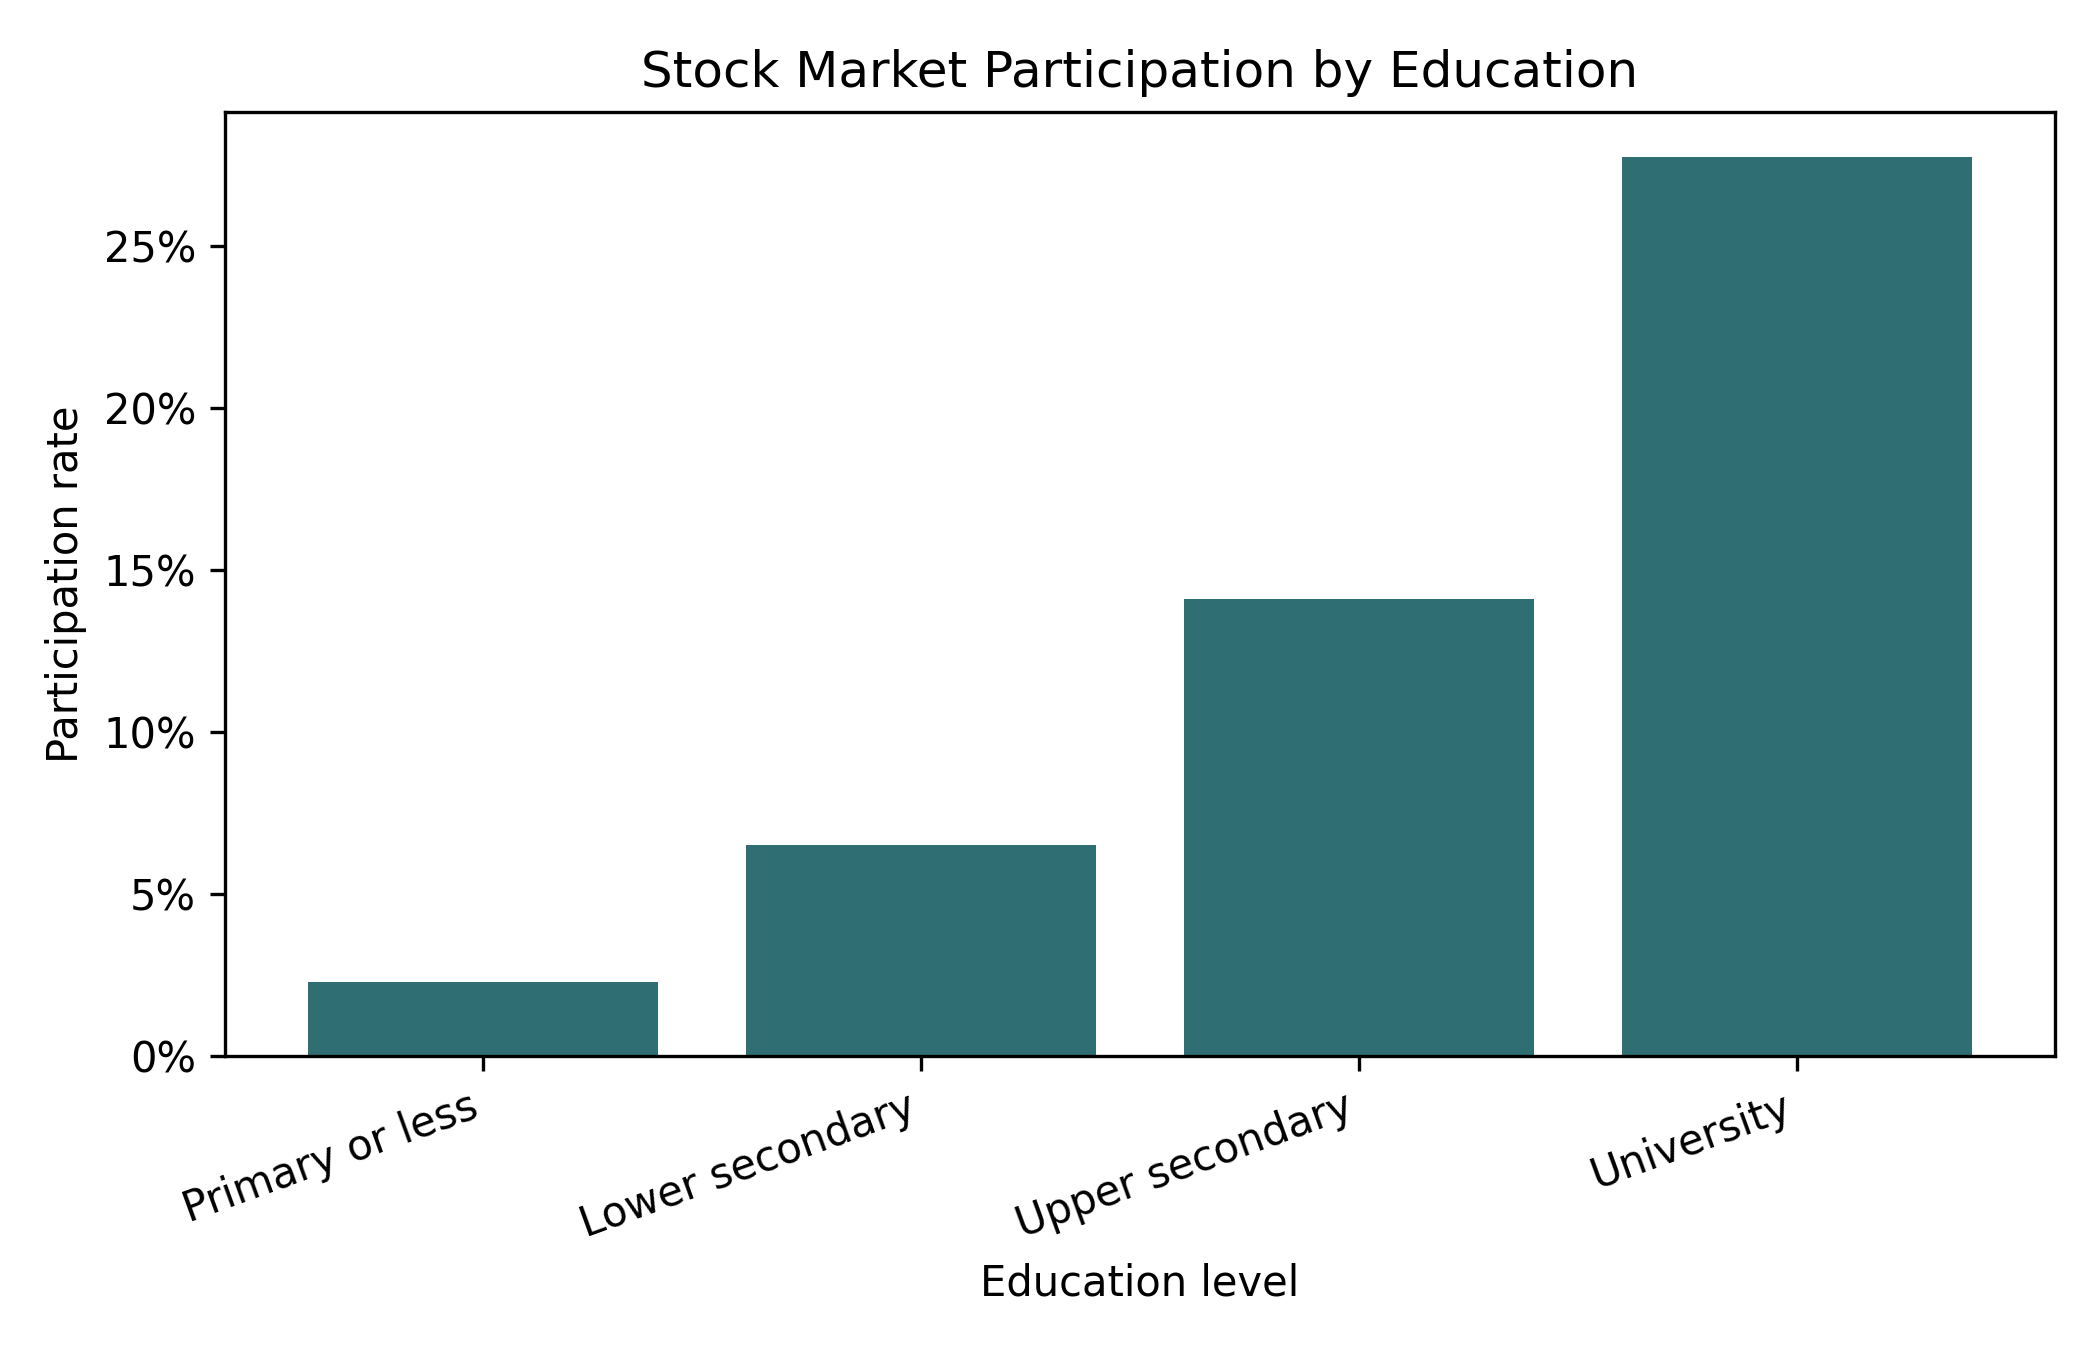
\includegraphics[width=0.85\textwidth]{output/participation_by_education.png}
\caption{Stock Market Participation by Education}
\end{figure}

\subsection{Participation by Region}

Participation also differs strongly by region.

\begin{table}[H]
\centering
\caption{Stock Market Participation by Region}
\begin{tabular}{lrr}
\toprule
\textbf{Region} & \textbf{Participation Rate} & \textbf{Median Income} \\
\midrule
North & 18.41\% & EUR 45,117 \\
Centre & 12.26\% & EUR 40,247 \\
South and Islands & 2.26\% & EUR 29,769 \\
\bottomrule
\end{tabular}
\end{table}

The North has the highest participation rate, while the South and Islands have a much lower rate. This may reflect regional differences in income, wealth, access to financial services, employment structure, and trust in financial institutions.

\subsection{Descriptive Results Summary}

The descriptive statistics reveal three important facts.

First, participation is low overall. A participation rate of 11.97 percent means that the majority of households do not own the selected risky financial assets.

Second, education is strongly related to participation. The participation rate increases monotonically across education groups. This pattern is consistent with the idea that education reduces informational barriers.

Third, geography matters. The participation rate in the North is much higher than in the South and Islands. Because this difference is large, region must be included as a control in the regression model.

\section{Regression Results}

\subsection{Main Probit Findings}

The probit results support the main hypothesis. The coefficient on log income is positive and statistically significant. This means that higher-income households are more likely to participate in the stock market, after controlling for education and demographic characteristics.

Education is also positive and statistically significant. Relative to households with primary education or less, households with lower secondary, upper secondary, and university education all have higher participation probabilities.

\begin{table}[H]
\centering
\caption{Main Probit Results for Stock Market Participation}
\begin{tabular}{lrrr}
\toprule
\textbf{Variable} & \textbf{Coefficient} & \textbf{Std. Error} & \textbf{Interpretation} \\
\midrule
Log income & 0.8072 & 0.0396 & Positive, significant \\
Lower secondary education & 0.3927 & 0.0829 & Positive, significant \\
Upper secondary education & 0.7051 & 0.0826 & Positive, significant \\
University education & 0.9563 & 0.0910 & Positive, significant \\
Centre & -0.2221 & 0.0381 & Lower than North \\
South and Islands & -0.8932 & 0.0593 & Much lower than North \\
Household size & -0.1916 & 0.0182 & Negative \\
Female household head & -0.2464 & 0.0318 & Negative \\
\bottomrule
\end{tabular}
\end{table}

Because probit coefficients are not direct percentage-point effects, the most useful interpretation comes from the average partial effects.

\subsection{Statistical Significance}

The main coefficients are statistically significant at conventional levels. In the output, the p-values for log income and the education categories are very small. This means that the estimated relationships are unlikely to be due to random sampling variation alone.

Statistical significance does not imply economic importance by itself. A coefficient can be statistically significant but small. In this project, however, the education and income effects are both statistically significant and economically meaningful. The average partial effects show that the size of the relationship is large enough to matter in practice.

\subsection{Average Partial Effects}

The average partial effects show the estimated change in probability.

\begin{table}[H]
\centering
\caption{Average Partial Effects}
\begin{tabular}{lr}
\toprule
\textbf{Variable} & \textbf{Average Partial Effect} \\
\midrule
Log income & 12.49 percentage points \\
Lower secondary vs primary or less & 3.98 percentage points \\
Upper secondary vs primary or less & 8.70 percentage points \\
University vs primary or less & 13.61 percentage points \\
\bottomrule
\end{tabular}
\end{table}

The university effect is especially important. Holding other variables constant, households with a university-educated head have a predicted participation probability that is 13.61 percentage points higher than households whose head has primary education or less.

The effect of log income is also large. A one-unit increase in log income is associated with a 12.49 percentage point increase in the probability of participation. Since log income changes are proportional, this result means that income growth is strongly connected to market participation.

\subsection{Predicted Probabilities}

The predicted-probability graph shows how participation changes with income for each education group.

\begin{figure}[H]
\centering
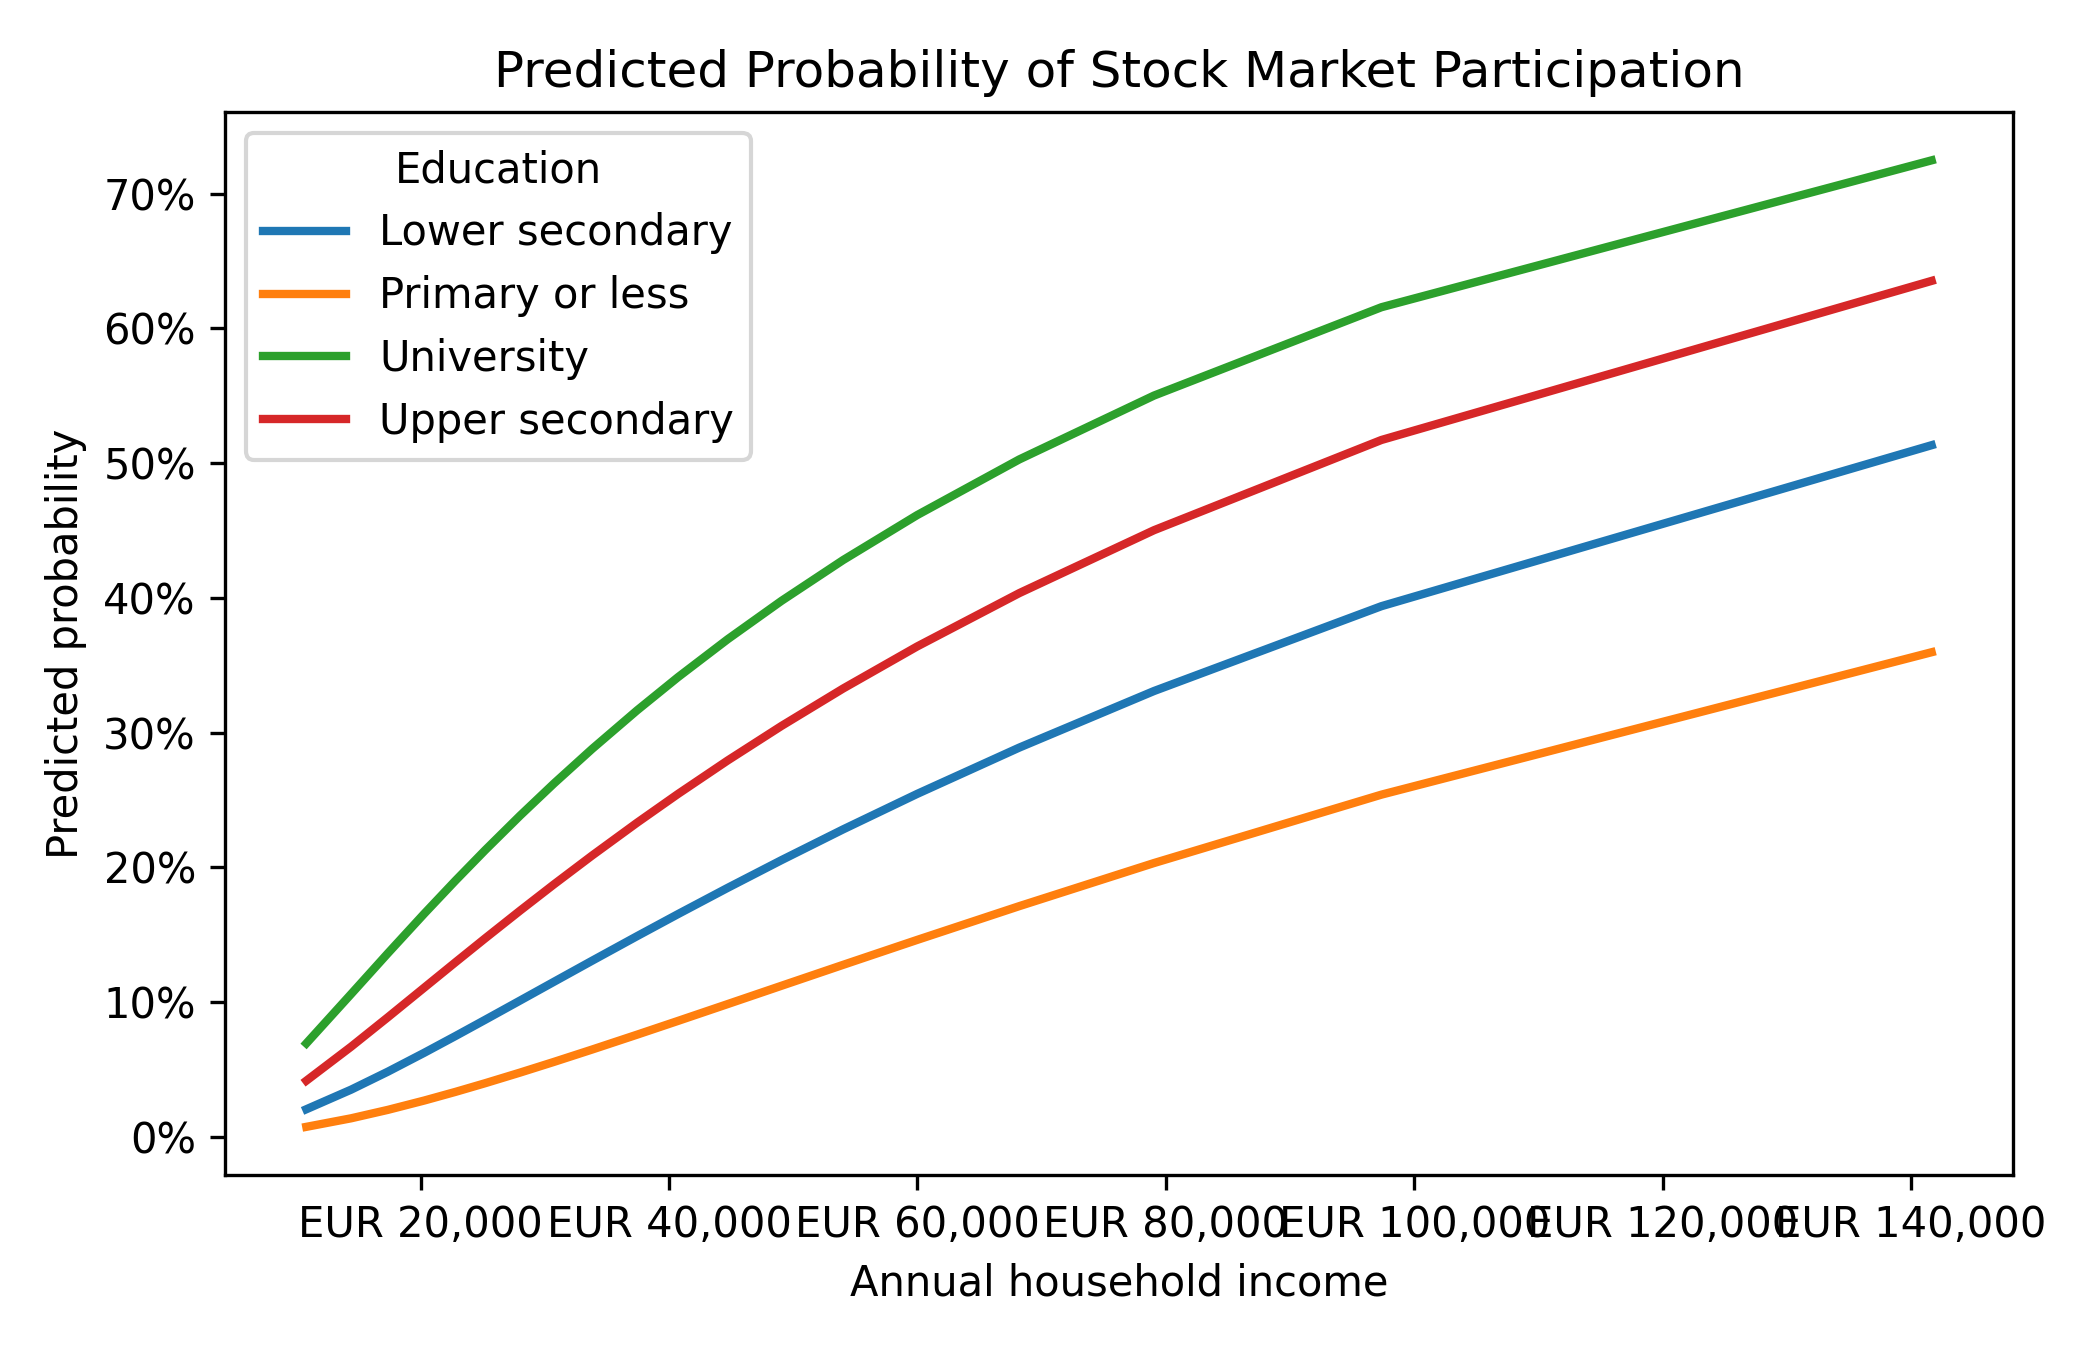
\includegraphics[width=0.85\textwidth]{output/predicted_probability_by_income_education.png}
\caption{Predicted Probability of Stock Market Participation by Income and Education}
\end{figure}

The figure shows two main patterns. First, predicted participation increases with income. Second, at any given income level, households with higher education have higher predicted participation. This means that education matters even after accounting for income.

\subsection{Robustness Interpretation}

The additional models for mutual funds/ETFs and direct listed stocks check whether the core story depends on the definition of participation. The preferred dependent variable is broad because it includes both direct and indirect participation. However, a narrower definition can still be informative.

If income and education remain positive in the narrower models, this supports the conclusion that socioeconomic status matters for different forms of market participation. If the coefficients become smaller for direct listed stocks, this may suggest that funds and ETFs are an easier entry point for households than direct stock ownership.

In the project output, the same general pattern appears: income and education are important predictors of participation. This gives confidence that the main result is not created only by one specific asset category.

\section{Interpretation}

\subsection{Income Effect}

The positive income effect is expected. Higher-income households are more likely to have savings available for investment after covering basic needs. They may also have better access to banks, financial advisors, and investment platforms. In addition, higher-income households may be more able to tolerate short-term financial losses.

\subsection{Education Effect}

The education effect may reflect several mechanisms. More educated households may understand financial products better, may be more familiar with risk diversification, and may have more confidence in using investment services. Education may also be correlated with financial literacy and trust in financial markets.

The results show that education is not only a proxy for income. Even after controlling for income, education remains strongly associated with participation. This suggests that informational and behavioral factors may matter.

\subsection{Regional Differences}

The negative coefficient for the South and Islands is large. This suggests that households in the South and Islands are much less likely to participate than households in the North. This may reflect regional differences in income, wealth, employment opportunities, local financial development, and financial culture.

\subsection{Practical Implications}

From a banking and wealth-management perspective, the findings suggest that financial institutions could focus on households with adequate income but low participation. These households may have the financial capacity to invest but may face barriers related to information, trust, or confidence.

Possible strategies include:

\begin{itemize}[leftmargin=*]
    \item clearer and simpler investment products;
    \item financial education programs;
    \item low-cost diversified funds;
    \item advisory services targeted at first-time investors;
    \item digital tools that explain risk and diversification.
\end{itemize}

\section{Business and Policy Implications}

\subsection{Implications for Banks and Wealth Managers}

The results suggest that financial institutions should not treat non-participating households as one homogeneous group. Some households do not participate because they have low income and limited savings. Others may have enough income to invest but do not participate because of informational, behavioral, or trust barriers.

The second group is especially important for banks and wealth managers. Middle- and high-income households with lower education may represent an underserved segment. They may benefit from simple diversified products, transparent fees, and advisory services that explain risk in plain language.

\subsection{Implications for Financial Education}

The strong education gradient suggests that financial education may matter. If formal education is related to financial knowledge, then improving financial literacy could reduce non-participation. However, financial education programs should be practical rather than abstract. Households need to understand concepts such as diversification, inflation, long-run returns, fees, and risk tolerance.

Financial education is unlikely to eliminate all participation gaps. Income, wealth, trust, and risk preferences also matter. Still, education-oriented interventions may help households make more informed decisions.

\subsection{Implications for Regional Inequality}

The very low participation rate in the South and Islands suggests that financial market participation is part of a broader regional inequality pattern. Lower participation may reduce long-run wealth accumulation if households miss opportunities for diversified investment returns. Policies that improve financial access and trust in underserved regions could therefore have long-run wealth implications.

\section{Limitations}

This project has several limitations.

First, the analysis is observational. The results show associations, not causal effects. For example, education is associated with participation, but the model does not prove that increasing education would mechanically increase participation.

Second, education is only a proxy for financial literacy. A household head may have high formal education but low financial knowledge, or low formal education but strong practical financial knowledge.

Third, the dependent variable measures whether the household owns risky financial assets, not how much it owns. A household with a small fund investment and a household with a large stock portfolio are both coded as participants.

Fourth, the analysis uses one survey wave. A panel analysis using multiple waves could study how participation changes over time.

Fifth, the project does not include risk preference variables. Risk tolerance is likely to affect stock market participation. If risk preferences are correlated with education or income, some part of the estimated relationship may reflect differences in risk attitudes.

Sixth, the project does not distinguish between small and large holdings. A participation dummy is useful for studying market entry, but it does not measure portfolio intensity. Future research could study the share of financial wealth invested in risky assets.

\section{Possible Extensions}

Several extensions could make the project stronger.

First, future work could use multiple SHIW waves and estimate whether the income and education effects are stable over time. This would show whether participation gaps are persistent or changing.

Second, the analysis could include wealth, not only income. Wealth may be even more directly related to investment capacity. A household with moderate income but high accumulated wealth may be more likely to participate than a household with high income but little wealth.

Third, the project could include financial literacy questions if available in a different SHIW wave. This would allow education and financial literacy to be separated.

Fourth, the project could estimate interaction effects between income and education. This would test whether education matters more for high-income households or whether income matters more for highly educated households.

Fifth, the analysis could compare direct stockholding with indirect participation through mutual funds and ETFs. This would be useful for understanding whether funds reduce the barriers to participation.

\section{Reproducibility}

Reproducibility is important because empirical results should be verifiable. This project keeps the analysis reproducible in several ways.

First, all code files are saved in the project folder. Second, the raw data folder path is explicitly shown in the code. Third, all output files are exported to the \texttt{output} folder. Fourth, a separate validation script checks the dataset construction. Fifth, a print script summarizes the results in a readable form.

The main workflow is:

\begin{enumerate}[leftmargin=*]
    \item run \texttt{analysis\_stock\_participation.R};
    \item run \texttt{print\_project\_results.R};
    \item review the exported tables and graphs in \texttt{output};
    \item compile this LaTeX report with \texttt{pdflatex}.
\end{enumerate}

This structure makes it possible to update the analysis if the data path changes or if the model specification is revised.

\section{Conclusion}

This project examined the determinants of household stock market participation in Italy using the 2022 Survey on Household Income and Wealth. The analysis focused on income and education as key predictors.

The results strongly support the hypothesis that income and education are positively associated with financial market participation. The weighted participation rate is only 11.97 percent, but it varies sharply by education. Participation is 2.30 percent among households with primary education or less and 27.76 percent among university-educated households.

The probit model confirms that these patterns remain after controlling for age, region, household size, and gender of the household head. Average partial effects show that university education is associated with a 13.61 percentage point higher participation probability compared with primary education or less.

Overall, the results suggest that stock market participation in Italy is strongly shaped by socioeconomic characteristics. Income provides the financial capacity to invest, while education may reduce informational and behavioral barriers. For financial institutions, the findings point to an opportunity to better serve households that have enough income to invest but remain outside financial markets.

\section{Bibliography}

\begin{itemize}[leftmargin=*]
    \item Bank of Italy. (2022). \textit{Survey on Household Income and Wealth 2022: Documentation and Stata Files}. Bank of Italy. \url{https://www.bancaditalia.it/statistiche/tematiche/indagini-famiglie-imprese/bilanci-famiglie/}
    \item Bank of Italy. (2022). \textit{Survey of Household Income and Wealth 2022: Documentation}. \url{https://www.bancaditalia.it/statistiche/tematiche/indagini-famiglie-imprese/bilanci-famiglie/documentazione/documenti/2022/Legen22_eng.pdf}
    \item Campbell, J. Y. (2006). Household finance. \textit{Journal of Finance}, 61(4), 1553--1604.
    \item Guiso, L., Haliassos, M., \& Jappelli, T. (Eds.). (2003). \textit{Stockholding in Europe}. Palgrave Macmillan.
    \item Guiso, L., Sapienza, P., \& Zingales, L. (2008). Trusting the stock market. \textit{Journal of Finance}, 63(6), 2557--2600.
    \item Haliassos, M., \& Bertaut, C. C. (1995). Why do so few hold stocks? \textit{Economic Journal}, 105(432), 1110--1129.
    \item Van Rooij, M., Lusardi, A., \& Alessie, R. (2011). Financial literacy and stock market participation. \textit{Journal of Financial Economics}, 101(2), 449--472.
\end{itemize}

\appendix

\section{Appendix: Files Created for the Project}

\begin{itemize}[leftmargin=*]
    \item \texttt{analysis\_stock\_participation.R}: main R analysis code;
    \item \texttt{analysis\_stock\_participation.py}: Python version used to generate outputs in this environment;
    \item \texttt{validate\_shiw\_data.py}: validation checks;
    \item \texttt{print\_project\_results.R}: R script to print results and code summary;
    \item \texttt{output/analysis\_dataset.csv}: final cleaned dataset;
    \item \texttt{output/probit\_results.csv}: regression results;
    \item \texttt{output/average\_partial\_effects.csv}: marginal effects;
    \item \texttt{output/participation\_by\_education.png}: education graph;
    \item \texttt{output/predicted\_probability\_by\_income\_education.png}: predicted probability graph.
\end{itemize}

\section{Appendix: Main R Commands}

To run the complete R analysis:

\begin{verbatim}
source("analysis_stock_participation.R")
\end{verbatim}

To print the results summary:

\begin{verbatim}
source("print_project_results.R")
\end{verbatim}

\end{document}
